%% This is an example first chapter.  You should put chapter/appendix that you
%% write into a separate file, and add a line \include{yourfilename} to
%% main.tex, where `yourfilename.tex' is the name of the chapter/appendix file.
%% You can process specific files by typing their names in at the 
%% \files=
%% prompt when you run the file main.tex through LaTeX.
\chapter{Návrh}
Hlavním cílem této práce je realizace anténní struktury pomocí technologii 3D tisku, a jelikož jako kterýkoliv jiný technologický proces má své omezení vyplívající z jeho principu, je vhodné tyto charakteristické vlastnosti brát v potaz již při návrhu.

Pokud se toto dodrží, minimalizuje se dopad nedokonalostí technologie, výrazně se zjednoduší realizace a splnění podmínky minimální post produkce produktu před jeho možným použitím.

\section{Trychtýřová anténa}
K návrhu trychtýřové antény lze přistoupit řadou různých způsobů, od odvození, přez aplikaci návrhových vzorů, až po využití moderních podpůrných software řešení typu Antenna magus. Jelikož tato práce je zaměřena zejména na výzkum možnosti uplatnění technologie 3D tisku pro výrobu této anténní struktury, byla zvolena cesta návrhu za podpory software Antena magus, který disponuje obsáhlou databází již ověřených parametrizovaných modelů.

Zvolené řešení umožnilo vyloučení návrhových chyb v porovnání s komplexními cestami a poskytlo optimální prvotní návrh, na kterém pak byly provedeny úpravy pro minimalizaci vlivů použité technologie. Další velmi významnou výhodou bylo poskytnutí plně parametrického modelu, což znamenalo znatelnou časovou úsporu, jak při návrhu, tak následné optimalizaci modelu.
\subsubsection{Vstupní model antény}
Geometrické rozměry optimálního trychtýře jsou následující:
\begin{itemize}
\item $a_1 = 110\,mm$ - Šířka ústí
\item $b_1 = 79\,mm$ - Výška ústí
\item $p = 228\,mm$ - Délka trychtýře
\item $plth = 0.15\,mm$ - Tloušťka stěny
\end{itemize}

\begin{figure}[!htbp]
\begin{center}
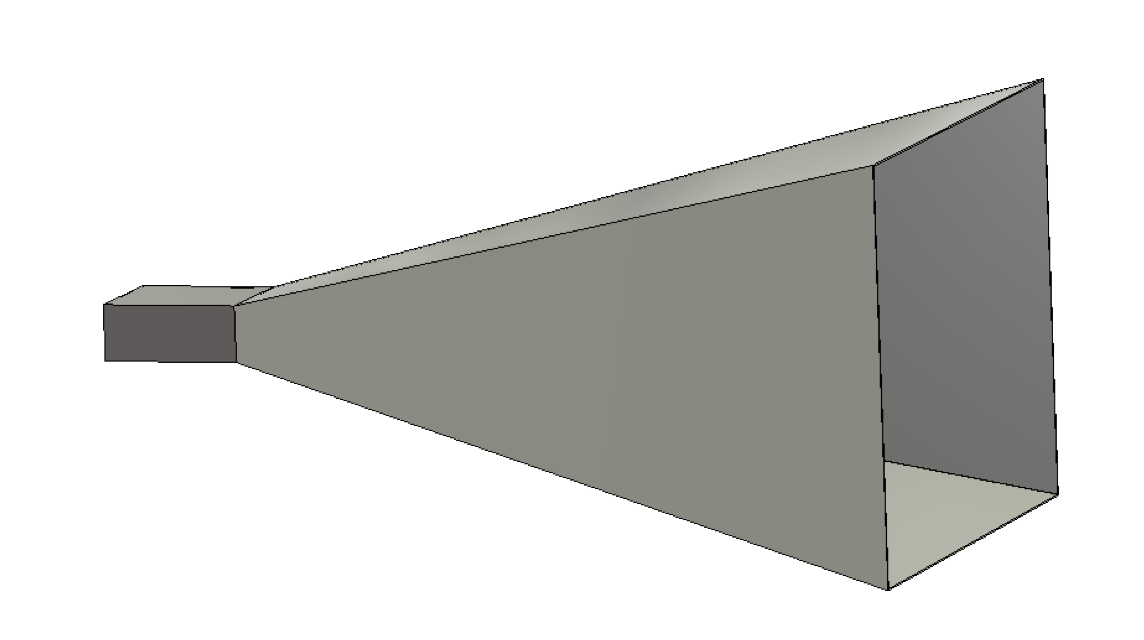
\includegraphics[width=9.5cm]{pics/HornOptimal}
\caption{Vstupní model antény}
\label{fig:hornOptimal}
\end{center}
\end{figure}

Jelikož ale standardně dostupné 3D tiskárny disponují pouze maximální možnou výškou výsledného produktu 200\,mm a průměrem trysky 0.4\,mm je patrné, že je třeba návrh struktury mírně zoptimalizovat.

Prvním parametrem, který je třeba změnit je délka trychtýře $p$. Je ale však nutné brát v potaz, že tento parametr je pouze délka samotného trychtýře. Jelikož ale potřebujeme i úsek vlnovodu, aby se střed trychtýře nacházel ve stejném prostředí, z důvodu stabilních podmínek, a samozřejmě bychom rádi strukturu osadili na vlnovod, musíme počítat s rezervou a nelze tedy nastavit  $p=200\,mm$.

Druhým parametrem je poté samozřejmě tloušťka stěny $plth$, která při hodnotě 0.15\,mm bude nerealizovatelná, jelikož je několikanásobně menší, než průměr vlastní trysky. Podobně jako u předchozího případu musíme počítat s rezervou, tentokrát však je ale podmínka více obecná. Pro udržení mechanické pevnosti struktur z důvodu chladnutí v průběhu procesu platí pravidlo alespoň dvojnásobné šířky extruze, tedy dle \ref{eq:MinWidth} (kde reprezentuje $W_{MIN}$ minimální šířku stěny v mm a $D_{nozzle}$ průměr trysky v mm) minimum $plth = 0.9\,mm$

\begin{equation}
W_{MIN} = 2*(D_{nozzle}+0.05) ; [mm, mm]
\label{eq:MinWidth}
\end{equation}

\subsubsection{Optimalizovaný model antény}
Po přiblížení se k výše uvedených optimalizačních cílů dostaneme následující parametry struktury:
\begin{itemize}
\item $a_1 = 110\,mm$ - Šířka ústí
\item $b_1 = 79\,mm$ - Výška ústí
\item $p = 140\,mm$ - Délka trychtýře
\item $plth = 1.45\,mm$ - Tloušťka stěny
\end{itemize}
Zde však nebyla volba zejména $plth = 1.45\,mm$ zcela optimální, aby bylo by možné v případě komplikací při procesu použít například $D_{nozzle} = 0.6\,mm$ 

Kde poté na srovnání \ref{fig:hornCompare} jsou viditelné nepatrné rozdíly pouze zkráceného (A), zkráceného s realizovatelnou šířkou stěny (B), včetně skutečně optimální (C) a zkráceného s realizovatelnou šířkou stěny a zavedenou udávanou vodivostí plánovaného materiálu na realizaci (D) trychtýře. Samotný vliv zkrácení trychtýře je již uveden na \ref{fig:HornLenDep}.

\begin{figure}[!htbp]
\begin{tikzpicture}[scale=1.4]
\begin{axis}[
    xlabel={Angle /\,$^\circ$},
    ylabel={Amplitude /\,dB},
    minor tick num=10,
    minor grid style={gray!25},
  	major grid style={black!50},
  	xmin=-180,xmax = 180,
  	%ymin=-120, ymax=-60,
    grid=both
]
\addplot [no markers, thick, blue] table [col sep=tab, y=Ae140thin] {hornSim.dat};
\addplot [no markers, thick, green] table [col sep=tab, y=Ae140thick] {hornSim.dat};
\addplot [no markers, thick, red] table [col sep=tab, y=Ae140thickOpt] {hornSim.dat};
\addplot [no markers, thick, orange] table [col sep=tab, y=Ae140thCond] {hornSim.dat};
\legend{A,B,C,D};
\end{axis}
\end{tikzpicture}
\caption{Řezy směrových charakteristiky v E rovině, kde: \textbf{A}-$p=140\,mm$, \textbf{B}- $plth=1.45\,mm$, \textbf{C}-$plth=0.9\,mm$, \textbf{D}- $plth=1.45\,mm$; $G=133.3\,S/m$}
\label{fig:hornCompare}
\end{figure}

\begin{figure}[!htbp]
\begin{center}
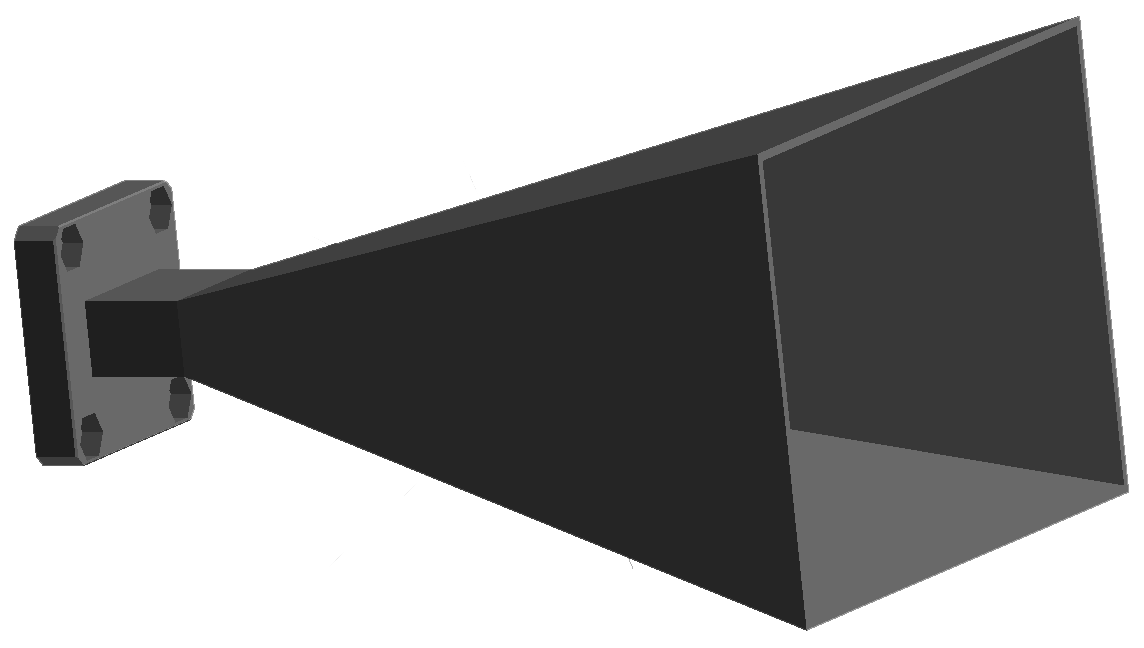
\includegraphics[width=9.5cm]{pics/HornFinal}
\caption{Výsledný model trychtýřové antény včetně příruby na vlnovod}
\label{fig:HornFinal}
\end{center}
\end{figure}

\subsubsection{Optimalizovaný model antény pro možnost post-produkce}
Uvažujeme-li aktuální reálné parametry, vliv technologie realizace a další proměnné, je velmi pravděpodobné, že pro praktické použití nebude smysluplné. Nicméně mohou postačovat pro následnou post-produkci, která při použití standartních materiálů je velmi komplikovaná, jako například pokovení.

Budeme-li chtít navrhnout strukturu pro tento postup, musíme model optimalizovat dále, jelikož i technologie následného pokovení má svá úskalí, jako například obtížné pokovení uvnitř dutin, vlnovodů. Zejména obtížné pokovování dutin je velmi významné omezení, pokud naše struktura je právě trychtýř a stejnoměrné pokovení uvnitř je zásadní.

Toto však snadno opět využitím technologie 3D tisku snadno vyřešit, v porovnání s úpravou pokovovacího procesu (nikoliv jeho parametrů). Tedy řezem středu trychtýře v E rovině, pro minimální ovlivnění povrchových proudů vnější stranou trychtýře a lehkého potlačení zadního laloku \ref{fig:hornCompareAssy}, a po následném pokovení mechanickým spojem. 

\begin{figure}[!htbp]
\begin{center}
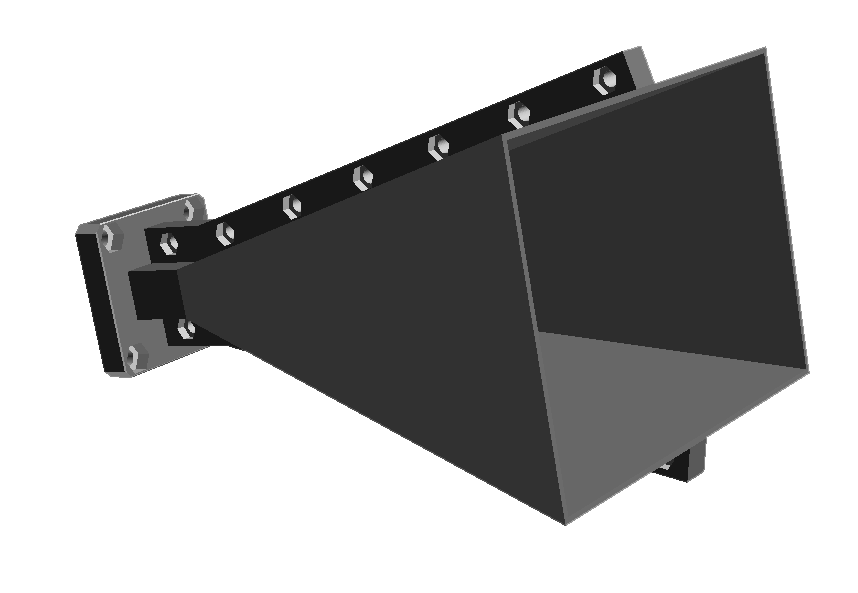
\includegraphics[width=9.5cm]{pics/HornAssy}
\caption{Výsledný model trychtýřové antény včetně příruby na vlnovod a následné sestavení}
\label{fig:HornAssy}
\end{center}
\end{figure}

\begin{figure}[!htbp]
\begin{tikzpicture}[scale=1.4]
\begin{axis}[
    xlabel={Angle /\,$^\circ$},
    ylabel={Amplitude /\,dB},
    minor tick num=10,
    minor grid style={gray!25},
  	major grid style={black!50},
  	xmin=-180,xmax = 180,
  	%ymin=-120, ymax=-60,
    grid=both
]
\addplot [no markers, thick, blue] table [col sep=tab, y=Ae140thickPrir] {hornSim.dat};
\addplot [no markers, thick, green] table [col sep=tab, y=Ae140thickAssy] {hornSim.dat};
\legend{A,B};
\end{axis}
\end{tikzpicture}
\caption{Řezy směrových charakteristiky v E rovině, kde: \textbf{A} - Původní optimalizovaný trychtýř, \textbf{B} - Trychtýř s přírubami na sestavení}
\label{fig:hornCompareAssy}
\end{figure}

\section{Extrakce dielektrických parametrů}
Jak již víme, pro účely této práce byla zvolena transmisní/reflexní metoda, jejiž princip je odvozen z charakteristického popisu odrazů a transmise při vložení vzorku do vedení. Cest, kterými se vydat, je ale velké množství, ať již odlišené dle volby vedení (koaxiální, vlnovodné), nebo zaměřujíc se na minimalizaci chyby určení specifických materiálů, je tedy nutno vybrat korektní implementaci metody. Jelikož našim cílem je aplikovat technologii 3D tisku, ideální aplikace je právě na metalický vlnovod z důvodu jednoduchosti realizace.

Abychom zajistili následnou možnost použití extrahovaných parametrů, zejména pro návrh anténní čočky, je nezbytné materiál charakterizovat v použitém kmitočtovém pásmu vlnovodu R100, tedy 8.2 - 12.5\,GHz.

Na základě definovaného kmitočtu a použité metody je nutno navrhnout výplně vlnovodu, které budou následně podrobeny měření \ref{fig:ExtractBlock}. Pro přesnou extrakci parametrů je velmi důležité zachovat celkovou délku systému $L$ a udržení měřeného vzorku ve středu pro minimalizaci fázové chyby, tedy v případě kratšího vzorku symetricky doplnit úseky vlnovodu. Dalším důležitým parametrem pro extrakci přesných dat je vhodné, aby útlum měřených vzorků byl alespoň 3\,dB, od čehož se bude odvíjet celková délka vkládaných vzorků.

\begin{figure}[!htbp!]
\begin{center}
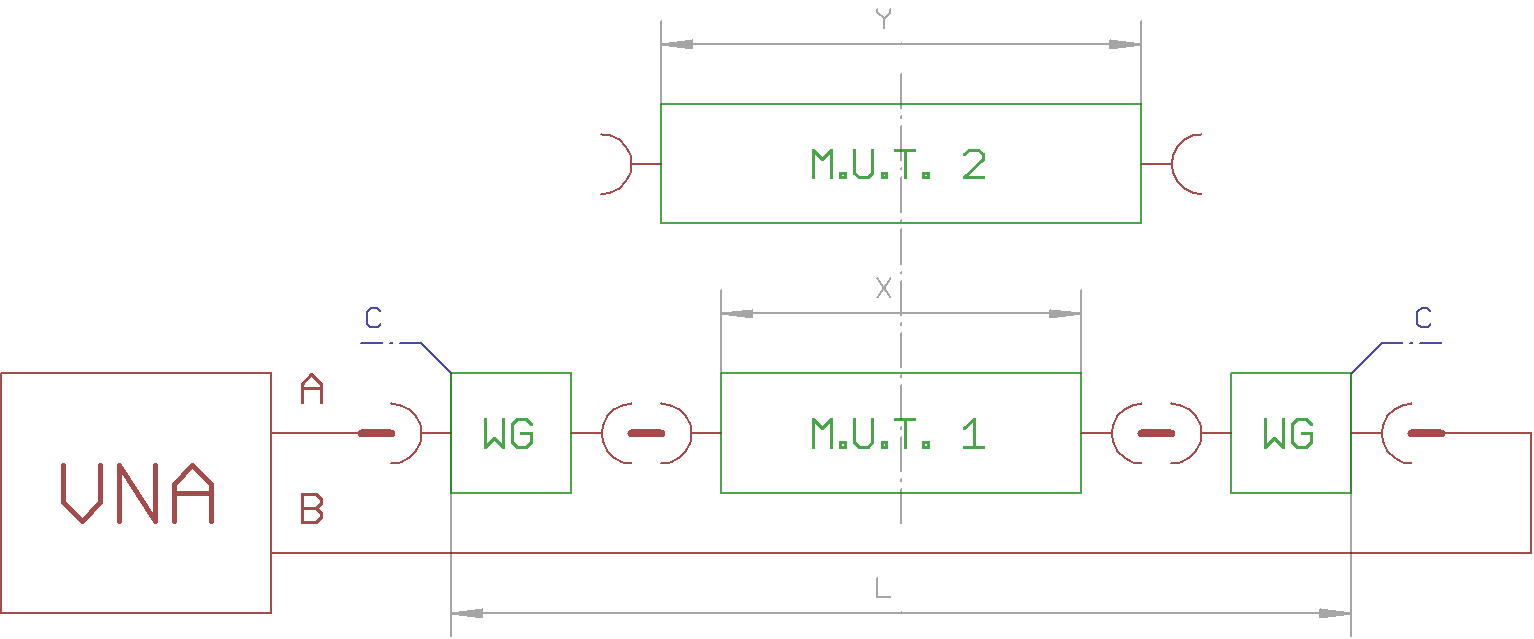
\includegraphics[width=9.5cm]{pics/ExtractBlock}
\caption{Blokové schéma transmisní/reflexní extrakce dielektrických parametrů}
\label{fig:ExtractBlock}
\end{center}
\end{figure} 



\section{Anténní čočka}
Na základě znalosti "vodivých" materiálů a jejich charakteru byl zvolen dielektrický typ čočky, konkrétně plano-konvexní čočka zejména kvůli vyšší předvídatelnosti chování dielektrických materiálů po průchodu technologickým procesem.
Jak již víme, k návrhu anténní čočky, lze přistupovat podobně jako k návrhu čočky optické.
Aby čočka splňovala svojí funkci transformace kulové vlny na rovinnou v dané aplikaci, je nutné zvolit pro následný návrh ohniskovou vzdálenost $F$ a průměr čočky $D$, které přímo lze spočítat na základě znalosti geometrických rozměrů antény.
Jako ohniskovou vzdálenost čočky je vždy nutné určit tak, aby zdroj byl právě v tomto bodě pro zajištění maximálně rovinné vlny. Rozhodneme-li se umístit čočku přímo na ústí struktury, musí být ohnisková vzdálenost právě rovna $p_1$. Za použití základní geometrie lze odvodit vztah \ref{eq:lensF}, kde poté vychází $F = 160\,mm$
\begin{equation}
F = p + \frac{\frac{b_1}{2}-(tg(\psi) p) }{tg(\psi)} ; [m, m, m]
\label{eq:lensF}
\end{equation}
Jelikož je důležité, aby čočka zároveň překrývala celou plochu ústí trychtýře, a příliš nepřesahovala, z důvodu minimalizace časové náročnosti realizace a objemu materiálu, lze její průměr vypočítat ze vztahu \ref{eq:lensDia}, kde po dosazení vychází $D = 136\,mm$.
\begin{equation}
D = \sqrt{a_1^2+b_1^2} ; [m, m, m]
\label{eq:lensDia}
\end{equation}
Posledním nezbytným parametrem pro finální je poloměr zakřivení čočky $R$. Tento zbývající parametr lze na základě známého návrhového pravidla \ref{eq:lensRad}, kde $\epsilon_r-lens$ je relativní permitivita materiálu čočky a $\epsilon_r-space$ relativní permitivita prostředí, po dosazení, a samozřejmě předchozí extrakce dielektrických parametrů materiálu, ze kterého bude následně čočka vytvořena, dospět k $R = 192\,mm$.
\begin{equation}
R = (\epsilon_{r-lens} - \epsilon_{r-space})F ; [m, -, -, m]
\label{eq:lensRad}
\end{equation}

\begin{figure}[!htbp]
\begin{center}
\includegraphics[width=9.5cm]{pics/LensDesign}
\caption{Návrh čočky}
\label{fig:LensDesign}
\end{center}
\end{figure}

\begin{figure}[!htbp]
\begin{center}
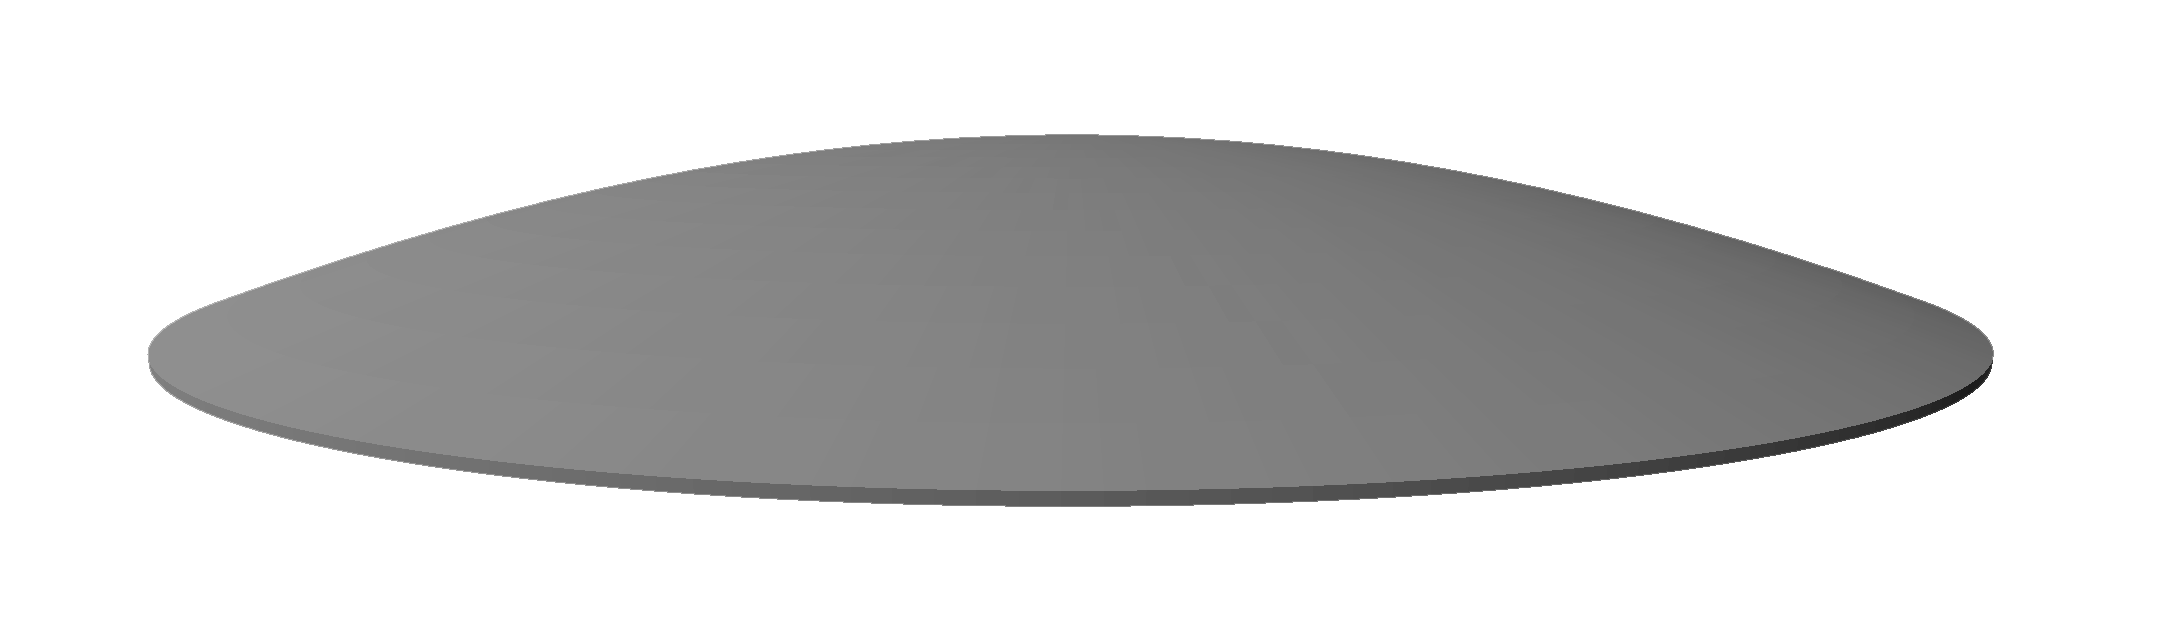
\includegraphics[width=9.5cm]{pics/LensModel}
\caption{Výsledný model čočky}
\label{fig:LensFinal}
\end{center}
\end{figure}

\begin{figure}[!htbp]
\begin{center}
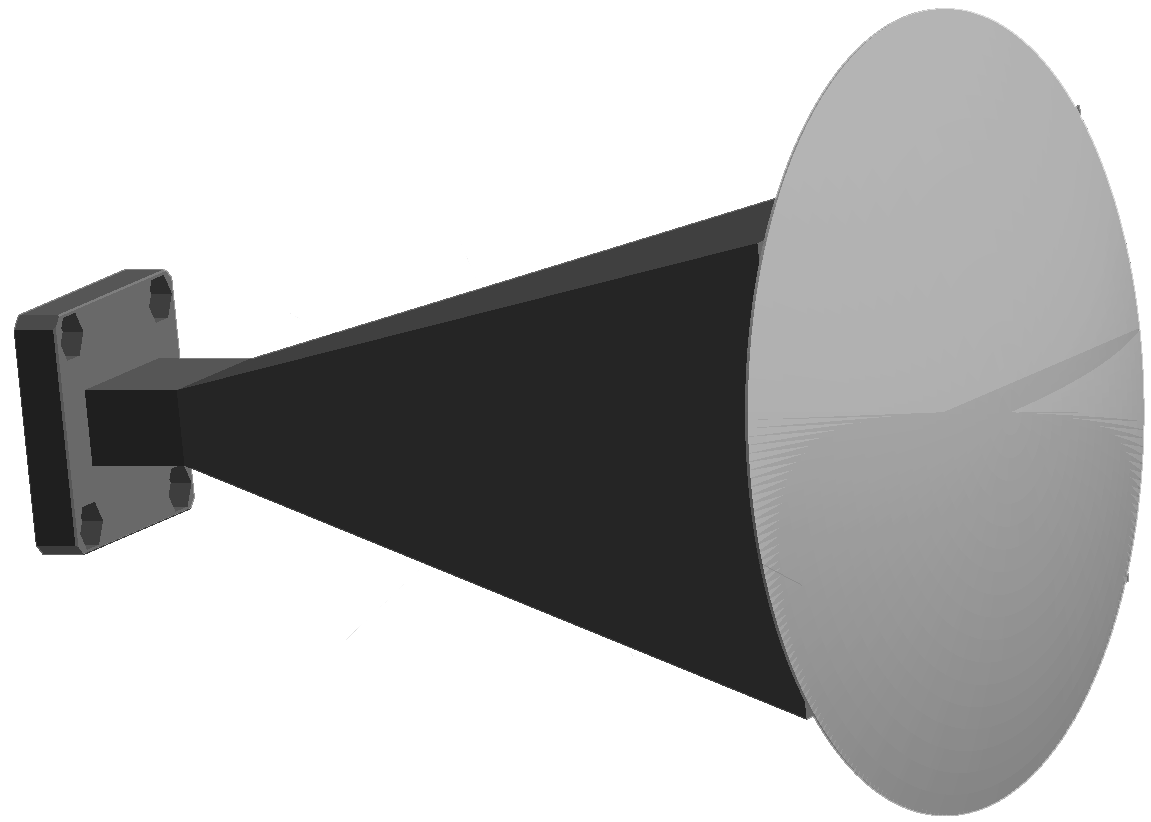
\includegraphics[width=9.5cm]{pics/HornFinalLens}
\caption{Výsledný model trychtýřové antény včetně čočky}
\label{fig:HornFinalLens}
\end{center}
\end{figure}

